The analysis of stoichiometric networks is relatively simple since it results in a linear system, where the vector $\vec{S}$ represents the metabolites and $\vec{\vec{N}}$ (stoichiometric matrix) the connectivity of the network.
\begin{figure}[H]
\begin{multicols}{2}
\begin{figure}[H]
\begin{tikzpicture}
\def\k{1.5}
\node[name=a] at (0,0){$A$};
\node[name=b] at (\k,\k){$B$};
\node[name=c] at (2*\k,\k){$C$};
\node[name=d] at (2*\k,-\k){$D$};
\node[name=f1] at (3*\k,\k){};
\node[name=f2] at (3*\k,-\k){};
\node[name=s] at (-\k,0){};
\draw[->,shorten <= 2pt, shorten >= 2pt] (s)--(a)node[midway,above]{$R_1$};
\draw[->,shorten <= 2pt, shorten >= 2pt] (a)--(b)node[midway,above left]{$R_2$};
\draw[->,shorten <= 2pt, shorten >= 2pt] (b)--(c)node[midway,above]{$R_3$};
\draw[->,shorten <= 2pt, shorten >= 2pt] (c)--(f1)node[midway,above]{$R_6$};
\draw[->,shorten <= 2pt, shorten >= 2pt] (c)--(d)node[midway,right]{$R_5$};
\draw[->,shorten <= 2pt, shorten >= 2pt] (a)--(d)node[midway,above right]{$R_4$};
\draw[->,shorten <= 2pt, shorten >= 2pt] (d)--(f2)node[midway,below]{$R_7$};
\end{tikzpicture}
\end{figure}\columnbreak
\begin{equation*}
\leadsto \vec{\vec{N}}=\begin{pmatrix} 1 & -1 & 0 & -1 & 0 & 0 & 0 \\ 0 & 1 & -1 & 0 & 0 & 0 & 0 \\ 0 & 0 & 1 & 0 & -1 & -1 & 0 \\ 0 & 0 & 0 & 1 & 1 & 0 & -1 \end{pmatrix}
\end{equation*}
\end{multicols}
\end{figure}
\noindent $\pm 1$ represent incoming (outgoing) fluxes. Here, we consider that one molecule creates one product. If two or more molecules would be needed, one would have to assign the fluxes accordingly.\\
The time evolution of the network is given by:
\begin{equation*}
\underset{\text{metabolites}}{\dot{\vec{S}}}=\underset{\text{stoichiometric matrix}}{\vec{\vec{N}}}\cdot\underset{\text{Fluxes between pools (nodes)}}{\vec{R}}
\end{equation*}
The stationary state is given by a set of linear equations of the kind: 
\begin{equation*}
0=N_{i1}R_1+N_{i2}R_2+\cdots +N_{iM}R_M
\end{equation*}
\subsubsection{Reconstruction of metabolic networks}
\begin{itemize}[label={$\to$}]
\item the reconstruction of (metabolic) networks in case of unknown edges is very labor intensive
\item Metabolites can be obtained with mass-spectroscopy
\item Pathways can be obtained from the presence of genes, homologies with other organisms etc.
\item The combined knowledge is used in order to fill the missing links
\end{itemize}
\subsubsection{Metabolic control analysis (MCA)}
\underline{Traditional view}: Every pathway has one limiting step which controls the output of the pathway\\
\underline{MCA}: Shared control replaces rate-limiting steps, i.e. every step in the pathway contriubutes to the control of the steady state flux.\\
\underline{Formal analysis} via control-coefficients and so called "{}elasticities"{}
\subsubsection{Generic metabolic pathway}
\begin{equation*}
\underset{\text{Input}}{I}\underset{V_1}{\overset{\overset{\overset{\text{enzyms}}{\downarrow}}{E_1}}{\to}}S_1\underset{V_2}{\overset{E_2}{\to}}S_2\underset{\underset{\underset{\text{reactions}}{\uparrow}}{V_3}}{\overset{E_3}{\to}}S_3 \cdots \to S_{n-1}\underset{V_n}{\overset{E_n}{\to}}\underset{\text{Output}}{O}
\end{equation*}
Steady state:
\begin{itemize}[label={\textbullet}]
\item All concentrations are constant, i.e. $\dot{I}=\dot{S}_i=\dot{O}=0$
\item All reaction rates must be the same $V_1=V_2=\cdots V_n$ where $J$ denotes the overall flux (conservation of mass)
\end{itemize}
Small pertubations: We are interested in small pertubations of the steady state and ask which reaction rates $v_i$ and metabolic concentrations have the strongest impact.\\
We characterize this by the following quantities:
\begin{equation*}
c_{V_i}^J=\frac{v_i}{J}\frac{\partial J}{\partial v_i}=\frac{\partial\ln(J)}{\partial\ln(v_i)}\qquad (\text{flux control coefficient})
\end{equation*}
The flux control coefficient measures the relative change of the flow via $v_i$.
\subsubsection{Metabolite Control Coefficient}
\begin{equation*}
c_{v_i}^{S_k}=\frac{v_i}{S_k}\frac{\partial S_k}{\partial v_i}=\frac{\partial\ln(S_k)}{\partial\ln(v_i)}
\end{equation*}
The influence of an enzyme on a flux or on a metabolite concentration can be very different. The impact of $S_k$ on $v_i$ is measured by the \textbf{elasticity coefficient}
\begin{equation*}
\epsilon_{S_k}^{v_i}=\frac{S_k}{v_i}\frac{\partial v_i}{\partial S_k}=\frac{\partial\ln(v_i)}{\partial\ln(S_k)}
\end{equation*}
One can show that $\sum\limits_{i=1}^{n+1}c_{v_i}^J=1$ and $\sum\limits_{i=1}^{n+1}c_{v_i}^{S_k}=0$\\
This relation is useful in order to determine whether all reactions of the patway have been detected.
\subsubsection{Example}
\begin{figure}[H]
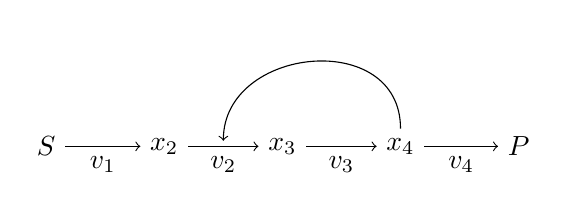
\begin{tikzpicture}
\def\k{1.5}
\node[name=s] at (0,0){$S$};
\node[name=x2] at (\k,0){$x_2$};
\node[name=x3] at (2*\k,0){$x_3$};
\node[name=x4] at (3*\k,0){$x_4$};
\node[name=p] at (4*\k,0){$P$};
\draw[->] (s)--(x2)node[midway,below]{$v_1$};
\draw[->] (x2)--(x3)node[midway,name=v2,below]{$v_2$};
\draw[->] (x3)--(x4)node[midway,below]{$v_3$};
\draw[->] (x4)--(p)node[midway,below]{$v_4$};
\draw[->,shorten >= 2pt] (x4) .. controls +(0,\k) and +(0,\k) .. (v2)node[midway,above]{$\circleddash$};
\end{tikzpicture}
\end{figure}
We consider a linear pathway with feedback. The following elasticities are known a priori.
\begin{equation*}
\epsilon_{x_2}^{v_1}=-\num{0.9};\ \epsilon_{x_2}^{v_2}=\num{0.5};\ \epsilon_{x_3}^{v_2}=-\num{0.2};\ \epsilon_{x_3}^{v_3}=\num{0.7};\ \epsilon_{x_4}^{v_2}=-1;\ \epsilon_{x_4}^{v_4}=\num{0.9}
\end{equation*}
The other elasticities are $\num{0}$.\\
Now we can use the identity $\sum\limits_{i=1}^wc_{v_i}^{J}\epsilon_{s_k}^{v_i}=0$ in order to determine all flux coefficients; e.g:
\begin{equation*}
c_{v_1}^{J}\epsilon_{x_2}^{v_1}+c_{v_2}^J\epsilon_{x_2}^{v2}=-\num{0.9}c_{v_1}^J+\num{0.5}c_{v_2}^J=0\qquad c_{v_4}^J = \num{0.38}
\end{equation*}
Solving the set of equations, we get:
\begin{equation*}
c_{v_1}^J=\num{0.19},\ c_{v_2}^J=\num{0.34},\ c_{v_3}^J=\num{0.10}
\end{equation*}
The information can be used in order to identify the bottle necks of the pathway and manipulate, e.g. the enzyme concentration of binding affinity to reduce the inhibition effects.
